\lecdate{24.05.2017}
\section{Grundlagen}
\subsection{Motivation}
\subsubsection*{Beispiele für deadlockgefährdete Abläufe}
\slides{05-deadlocks}{2}
(wenn beide Prozesse ihren ersten Semaphor sperren, bleiben sie beide beim sperren des zweiten stehen und schlafen unendlich
\subsection{Deadlock vs Livelock}
\slides{05-deadlocks}{3}

\section{Eintrittsbedingungen}
\slides{05-deadlocks}{4}
($\to$ potentielle Prüfungsfrage)

\subsection{Dynamik des Deadlockeintritts}
\subsubsection*{Beispiel: 3 Prozesse konkurrieren um 3 Ressourcen R, S, T}
\slides{05-deadlocks}{5}
\subsubsection*{Lehren aus diesem Beispiel:}
\slides{05-deadlocks}{6}
\subsection{Ressourcenzuteilungsgraph}
\slides{05-deadlocks}{7}
\begin{center}
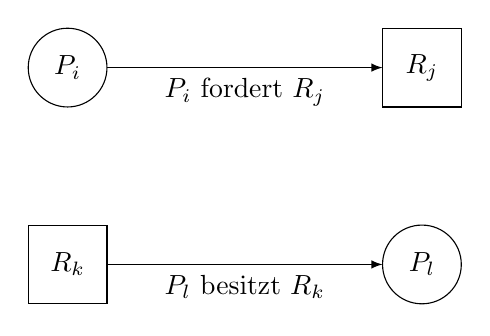
\begin{tikzpicture}
\draw  (0,0)node{$P_i$} circle (0.5);
\draw  (4,-0.5) rectangle node{$R_j$} (5,0.5);
\draw [-latex] (0.5,0) -- node[below = .5]{$P_i$ fordert $R_j$} (4,0);

\draw  (-0.5,-3) rectangle node{$R_k$} (0.5,-2);
\draw  (4.5,-2.5)node{$P_l$} circle (0.5);
\draw [-latex] (0.5,-2.5) -- node[below = .5]{$P_l$ besitzt $R_k$} (4,-2.5);
\end{tikzpicture}
\end{center}
\subsubsection*{Beispiel}
\slides{05-deadlocks}{8}

\section{Strategien zur Deadlock-Behandlung}
\slides{05-deadlocks}{9}
\subsection{Ignorieren von Deadlocks -- Vogel-Strauß-Algorithmus}
\slides{05-deadlocks}{10}
MTBF: Mean Time Before Failure
\subsection{Erkennen und Beheben von Deadlocks}
\subsubsection{Erkennung}
\slides{05-deadlocks}{11}
\subsubsection{Algorithmus zum Erkennen eines Zyklus im RZG}
\slides{05-deadlocks}{12}
\subsubsection{Beschreibung mittels Belegungs- und Anforderungsmatrix}
\slides{05-deadlocks}{13}
$\to$ Effizienteres Verfahren zur Erkennung als über den RZG.
\subsubsection*{Beispiel}
\slides{05-deadlocks}{14}
\subsubsection{Algorithmus zur Erkennung von Deadlocks}
\slides{05-deadlocks}{15}
\subsubsection*{Beispiel}
\slides{05-deadlocks}{16}
$\vec{E}$: Spaltensumme von $\cR$.\\
Bei $\vec{A}$ wird von $\vec{E}$ subtrahiert: Die Spaltensummen von $\cC$!\bigskip\\
Prozesse die vollständig ablaufen können, geben ihre Ressourcen wieder zurück. Prüfe, ob alle Prozesse ablaufen können, nachdem fertige Prozesse ihre Ressourcen jeweils freigegeben haben!

\subsection{Zeitpunkt der Erkennung / Behebung eines Deadlocks}
\slides{05-deadlocks}{17}
Entzug einer Ressource Beispiel: Speicherblock auf Festplatte zwischenspeichern, Prozess anhalten, Speicher anderem Prozess geben und wenn der fertig ist, Speicherblock von Festplatte wieder zurück schreiben.\\
Rollback mit Checkpointing: Wie ein Auto-/Quicksave im FPS 

\subsection{Dynamisches Vermeiden}
\lecdate{31.05.2017}
\slides{05-deadlocks}{18}
\subsubsection*{Beispiel}
\slides{05-deadlocks}{19}
N fordert max. 5, hat schon 2, braucht also noch 3 -- die sind noch frei. Daher kann N durchlaufen und mit den freigegebenen Ressourcen kann auch M durchlaufen $\to$ ist also sicher.
\slides{05-deadlocks}{20}
Das ist nicht mehr sicher, da kein Prozess beendet werden kann (beide brauchen noch 3, können aber maximal 2 bekommen).
\subsubsection{Realisierungsverfahren}
\slides{05-deadlocks}{21}

\subsection{Statisches Verhindern}
\slides{05-deadlocks}{22}
\slides{05-deadlocks}{23}

\section{Ausblick}
\slides{05-deadlocks}{24}


